\documentclass[a4paper, 11pt]{article}
\setlength{\topmargin}{-0.5in}
\setlength{\textheight}{9.5in}
\setlength{\oddsidemargin}{-.1in}
\setlength{\textwidth}{6.5in}

\usepackage{multirow}
\usepackage{float}
\usepackage{array}
\usepackage[document]{ragged2e}

\usepackage{datetime}

\newdateformat{mydate}{\monthname[\THEMONTH] \THEYEAR}

\newcolumntype{L}{>{\centering\arraybackslash}m{3cm}}

\usepackage{graphicx}
\graphicspath{{images/}}

\begin{document}


\LARGE\title{User Modeling in search for People with Autism}

\LARGE\author{Author: \textbf{Esha Massand}, Supervisor: \textbf{Keith Mannock}\\
\\
Birkbeck, University of London\\Department of Computer Science and Information Systems\\\\\\Project report submitted in partial fulfillment of the requirement for the \\MSc in Computer Science\date{\mydate\today}
\\\
}

\normalsize


\maketitle


\section*{Abstract}
\begin{justify}
This project report presents the development of a prototype web application to assist users with Autism when they search the web. The developed system models user interactions with the search process into a user profile by integrating insights from the core features of autism into the model. The user profile is applied to a synthesis of three leading search engines, and the entire system is integrated with an infra-red user interface component to assist users with Autism during search.\\
\end{justify}


\begin{justify}
This project is substantially the result of my own work, expressed in my own words, except where explicitly indicated in the text. I give my permission for it to be submitted to a Plagiarism Detection Service. This proposal may be freely copied and distributed provided the source is explicitly acknowledged.
\end{justify}

\begin{verbatim}














\end{verbatim}

\begin{center}
word count (proposal text only) : 3294 words.
\end{center}

\clearpage
\tableofcontents
\clearpage

\section*{Abbreviations}
\begin{tabular}{l l }
API & Application Programming Interface\\
AQ & Autism Quotient\\
ASD & Autism Spectrum Disorder\\
DSM & Diagnostic and Statistical Manual\\
GCS & Google Custom Search\\
HCI & Human Computer Interaction\\
HTTP & Hypertext Transfer Protocol\\
JSON & JavaScript Object Notation\\
IDE & Integrated Development Environment\\
KWIC & Key Word In Context\\
LEAP & LEAP Motion Controller\\
REST & Representational state transfer\\
RIFT & Oculus Rift Virtual Reality Head Mounted Display\\
TDD & Test Driven Development\\
UI & User Interface\\
UX & User Experience\\
VR & Virtual Reality\\
\end{tabular}

\section*{Definitions}

\begin{tabular}{l p{15cm}  }
Autism & Autism is amongst the most common neurodevelopmental condition and it is currently estimated that 1/68 children meet criteria for Autism Spectrum \cite{CDC}. Autism is five times more common amongst boys than girls (1/42 boys, and 1/189 girls). According to the Diagnostic and Statistical Manual (2013), Autism is characterized by persistent and early deficits in reciprocal social interaction and repetitive behaviours. Individuals vary from high functioning to low functioning (along a spectrum), with behaviours emerging around 2 to 3 years of age.
\end{tabular}
\clearpage

\section{Introduction}\label{intro}

This project report presents the development and evaluation of a prototype web-browser based application to assist users with Autism when they search the web, hereafter referred to as Jellibeans \footnote{Jellibeans are a rainbow of colours, different sizes and shades, and the name represents the difference in style of processing of individuals with ASD.}. Jellibeans will run in a web browser and utilises gesture and hand movement data recorded using the Leap Motion Controller (LEAP). 

Individual characteristics of each user will be measured using a 50 item questionnaire, the Autism Quotient (AQ \cite{Baron Cohen et al}) which measures tendency towards autistic traits. A score of 32 or higher indicates a strong likelihood of Autism or Asperger syndrome (the questionnaire has a 79\% sensitivity score). Individuals who score highly on the AQ will be offered the current user model for their search. The questionnaire data will be stored in the user's Google+ profile????

In programmatic terms, Jellibeans is designed to implement a research-based user model in search. This itself is a considerable part of the current research project and involves the development of a rule engine to transform the idiosyncratic ??? nature of search queries formed by individuals with ASD to work with current available search engines. This development involved collecting and analysing search behaviour patterns from people with and without ASD and building a set of transformation rules given the features of search queries that are formed by individuals with ASD.

Jellibeans will also improve the search experience for users with ASD by going one step further and enabling motion controlled search using the LEAP motion controller. The interface will be dynamic as opposed to static and this afford many advantages over traditional search engine interfaces.

\subsection {User Models in Search}

\subsection {Rule and Transformation Engine}

\subsection {Motion Controlled Navigation in Search}


\section {Aims}
The goal of the project is to build a prototype search tool that assists users with Autism search and navigate the web. To acheive this goal, the aims of this work are:

To synthesise the search results from three search engines, Google, Bing and Yahoo. For search results returned by Google, the Custom Search API will be used in line with the Google terms of service (as `screen scraping', or copying the data directly from the website is prohibited). It is a RESTful api with a single method called list. The API method used was GET, and the response data is returned as a JSON type. The response consists of (1) the actual search result, (2) metadata for search like number of  results, alternative search queries, and (3) custom search engine metadata. The data model depends on \cite{opensearch}.
For Bing and Yahoo search results, JSoup (a Java HTML parser) will be used to identify the links from the resulting query. The JSoup HTML parser was considered more effient for retrieving search results, as it reduced the number of lines of code required to complete the task. 
Jsoup has its advantages over html parsing. It contains a class representing a list of nodes, `Elements', which implements Iterable to iterate over a list in an enhanced for loop.
The resulting links are written to text file which stores the links in a text file in the projects source directory.

The system aims to deliver relevant results to the user, but what is ``relevant"? Not all users or groups of users search in the same way, so it is important to consider user intention. The first part of the current project aimed to investigate the differences between search queries of people with and without Autism, and to use those findings to build a stereotyped user model (a user model that will infer characteristics about the user from their diagnostic information) for a person with autism. Users will have to register will Google+ ???, and report their diagnostic information in the aboutMe section of their profile ??? / complete the Autism Quotient Questionnaire and obtain a score of autistic-like traits. Using the Google+ API, Jellibeans will connect to Google+ and ask the user to signin/ agree to the web application accessing their data. JavaScript will be used to parse the text in the aboutMe section to check if the user has identified as a persn with autism, aspergers, ASD or not. The result is returned via the console (inspect) command. ??? 


\section {Method}
\subsection{Building a User Model into Search}\label{building the user model} 
Search queries usually fall into one of three broad categories.  `Do' queries which characterise transactions between the user and the search engine, for example when the user wants to do something such as buy a plane ticket or listen to a song. There are also `Know' type queries. These are informational queries for example, the name of a band or restaurant in London. The third broad category is `Go' type queries, which are navigational in nature, for example, searching for a particular home page on the web. 

There are many stages to the search process. After identifying the information need, the user must formulate a search query. The user must browse through results once the query has been entered into a search engine. The whole process can be repeated if the user is not satisfied. The stage at which the user model will have most possible impact is before results are returned to the user, that is, at the query formulation stage. It is this stage that the user model will be implemeted (stage 2 on Figure~\ref{search flow}).


\begin{center}
\begin{enumerate}
\item{Experience the need for an answer,
solution, or piece of information.}
\item{Formulate that need in a string of words and phrases, also known as “the query.”}
\item{Enter the query into a search engine.}
\item{Browse through the results for a match.}
\item{Click on a result}
\item{Scan for a solution, or a link to that solution.}
\item{If unsatisfied, return to the search results and browse for another link or ...}
\item{Perform a new search with refinements to the query}
\end {enumerate}
\label{search flow}

\hspace{1cm}
Typical user's search flow process \cite{seo}

\end{center}

\subsection{Data Collection}
To identify the features of the user model to build, I ran a study to collect example search queries on a set of informational needs from 33 participants. The participants were asked to give examples of search queries they would use to identify the name of a song they had heard (given the lyrics), or the name of a breed of a dog they had seen (given a picture of the dog). There were in total 10 search queries; the study was distrbuted widely via Surveymonkey.com \cite{surveymonkey} and can be seen in Appendix~\ref{AppendixA}. Participants were also asked to complete the Autism Spectrum Quotient 50-item questionnaire see Appendix~\ref{AQ}. The participants responses are analysed and reported back to surveymonkey.

The range of scores for the AQ is 0 to 50 with high scores indicating increased liklihood of autism-like traits. A score under 21 is a low to average result (many women average around 15 and men around 17). A score of 22-25 indicates autistic tendencies slightly above the population average. A score above 26 gives a borderline indication of high functioning autism, or aspergers. A score above 32 suggests a likelihood of Asperger syndrome or autism (sensitivity of test measure = 79\% \cite{Baron Cohen et al}). However although the AQ is a useful tool, it is by no means a form of diagnosis of autism. For the purposes of this study, individuals with scores equal to, and above 30 were interpreted as having `autistic-like traits'.

Participants were divided into two groups; low AQ scorers (scores below 30), and high AQ scorers (scores equal to and above 30). There were 26 low AQ scorers and 7 high AQ scorers. 


\subsection{Differences in Search Queries Between Users With and Without Autistic-like traits.}
I conducted a qualitative analysis on the search query strings from both low and high AQ scorer groups.

In both groups, Google was the prefered search engine by far, with all participants reporting that they used Google as a first choice. No one in the current sample used Yahoo or Bing. 
The low AQ scorer responses were analysed as a group. A `model' (or baseline) was generated using a frequency criterion of 40\% i.e., if 11 out of 26 respondents or more generated the same query string given an informational need, it was included in the model below. If two responses were equally as common, both are reported in the model. When a response indicated that the participant would do an image search, I was unable use those data. The results from the frequency analysis are presented below.

\begin{enumerate}
\item{You hear a song on the radio with the lyrics, ”Look at your children”, and you want to download it. What would you type into search on your favourite search engine to find out what song it was?\\\textit{Look at your children song}. \\\textit{Look at your children lyrics}.}
\item{You’ve lost touch with an old school friend (you went to St. Mary’s School). What key words/queries would you use to find them?\\\textit{St. Mary’s School Year of X}.}
\item{How would you identify what this is using a search engine (pretend you don’t know what it is called). What key words/queries would you use?\\\textit{Star shaped brown plant}.}
\item{How would you find out the name of this famous person using a search engine? What key words/queries would you use?\\\textit{Brown hair famous young women}.}
\item{How would you identify what breed this animal is using a search engine? What key words/queries would you use?\\\textit{Small dog fluffy breed}.}
\item{Your friend and you can’t agree on how Thandie Newton pronounces her first name. How would you resolve this using a search engine?\\\textit{Thandie Newton pronunciation}.}
\item{What would you search for to identify this pattern’s name, and which country it originates from?\\\textit{Repeating square maze pattern border}.}
\item{How would you search for delay’s relating to your (imminent) flight to Paris?\\\textit{Flight number, carrier, Paris, airport, flight time}.}
\end{enumerate}

The following observations were made for the users in the high AQ group:
\begin{enumerate}
\item{Although high AQ scorers' for the most part, formed query strings accurately, there was increased use of idiosyncratic words in the query strings that were forumulated. This is in line with previous research that suggests that people with autism organise information in more subjective and individual ways \cite{subjective organisation}. For example, referring to the picture of the dog as `yorkie pooh'(not listed in frequency index), `aeroplane' (frequency of 8254 words per million) instead of plane (frequency of 33900 words per million) or flight (29535 words per million) , `miniature' (less than 4973 words per million) instead of small (185463 words per million). The idiosyncratic nature of the words is captured by their lower frequency of use in the English language. Search engines use term frequency to determine if a document is relevant to the users search query. If the frequency of words used to form search queries differs between low and high AQ scorers, so will the returned search results.}

\item{There were an increased number of imcompletely formed queries, in other words, in the high AQ group participants were more likely to miss off words in the query string. This was observed even though the sample size was much smaller in the high AQ group (7 people) compared to the low AQ group (26 people)). For example, when analysing the resuls from query 1 above, 2 out of 7 respondents in the high AQ group did not put `lyrics' or `song' in the search query when searching for the lyrics ``Look at your children". When these search strings are entered into Google, the results are very different (see Figure~\ref{someresults}), suggesting that Google is not performing well for the high AQ user group.

\begin{figure}[H]
\begin{center}
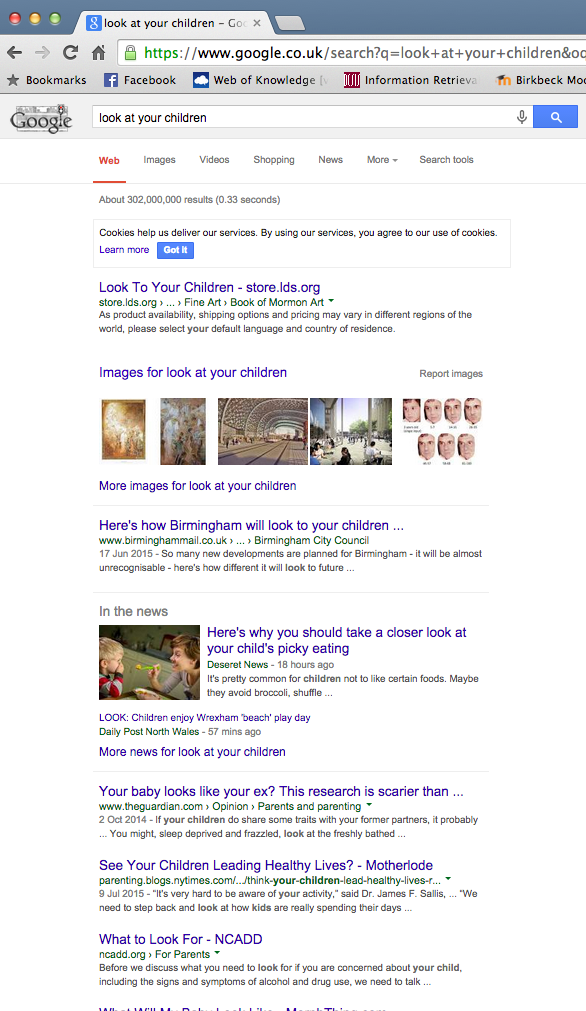
\includegraphics[scale=0.7]{lookAtUrChildren}\\
\end{center}
\end{figure}

\begin{figure}[H]
\begin{center}
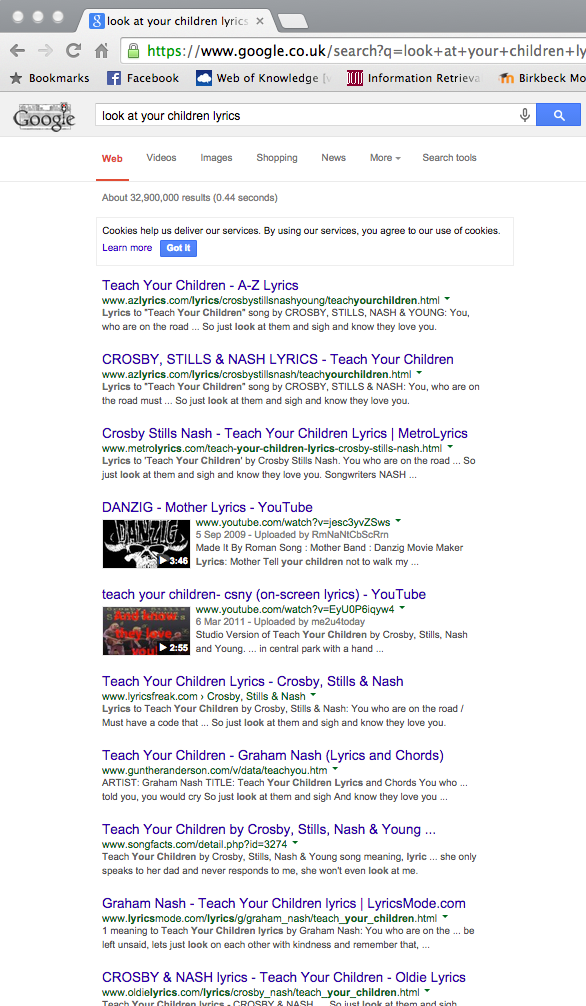
\includegraphics[scale=0.7]{lookAtUrChildrenLyrics}\\
\caption{High and low AQ scorers both formed search queries accurately, however there was an increased tendency to omit the word ``lyrics" in the high AQ group resulting in very different search results.}
\label{someresults}
\end{center}
\end{figure}
}

\item{One individual of the 7 individuals in the high AQ group demonstrated ambiguous use of third-person pronouns, which is characteristic of some individuals with Autism \cite{pronoun}. This includes using first names instead of `I' or `you'. This is particularly detrimental to search engine query strings because the use of names distrupts the term frequency - inverse document frequency weighting \cite{tfidf} of the search query and subsequently the results returned to the user.
}
 
\item{
For questions that were `social' in nature (e.g., featuring a face of a famous woman), 2 out of 7 individuals in the high AQ group indicated that these were types of queries that they would not normally be interested in, and so ``wouldn't bother asking it". This is, of course, in line with the characteristics of Autism according to \cite{DSM}. For these queries, it was more common for individuals in the high AQ group to include information in their search query string that was extraneous to the search question itself, compared to the low AQ group. For example, in query 4 above (which asked respondents to indicate how they would identify a famous person), 2 high AQ scorers included information about the woman's earing. Inevitably this `dilutes' the search query and results in reduced precision for the search engine.
}

\item{ 
Lastly there were more spelling errors and typographical errors in the high AQ group compared to the low AQ group.
}

\end{enumerate}
\subsection{Building the Jellibeans Transformation Rule Engine}
Given the set of observations above, the aims were to `transform' queries made by individuals in the high AQ group, using a set of rules (hence forth called the `rule engine', to queries that share greater overlap with those made by the low AQ group. 

From theoretical to concrete
Results of the data collection
Profile of users and user groups

\subsection{Implementation}
What was actually done
Classification of users
Feature uses
Storage of information


\subsubsection{Integrating Jellibean with Motion Controller Hardware}
LEAP motion controller and its use for the system.
Current Project’s Hardware Selection Process and Important Design Issues:
\begin{enumerate}
\item{Good timing correlates to a good meaning and User Experience.}
\item{The leap has options to ‘poll’ frames at a constant rate (to keep timing of movement accurate) which is important.}
\item{Cognitive ‘lag’ time. Each of our senses operates with a different lag time. Hearing has the fastest sense-to-cognition/understanding time, and surprisingly sight -- the slowest. If the devices interferes with the processing of the sense, it will confuse the combinatorial configuration of the senses, leading to misunderstandings in the meaning and a worse user experience.}
\item{Volume is important because this is a tool to be used with individuals with ASD, the device must have a low `volume’, i.e., the sensory experience cannot be overwhelming.}
\item{Load, by this I mean `cognitive' load is most desirable when not high. We do not want the device to be overwhelming in terms of it’s cognitive load.}
\item{Within the selection process, I did not just consider the physical design of the device, but also the way in which the devices manifests actions into behaviours. That is, how does the user engage behaviourally within the environment using the device? What about the physical sensation and its path towards a behavioural or emotional response? For example, can we program there to be an activity followed by a reward to reinforce the activity.}
\end{enumerate}


\subsection{Development and Implementation of Jellibean}
\subsection{API's and Development Tools}


\section{Result}
The transformations that were implemented


\section{Conclusion}
How does it compare to the original specification
This work has successfully completed aims XXX

\subsection{Signals of Quality Content}
I will test and evaluate the system. Testing will involve assessing the reliability and robustness of Jellibeans; the ease of its interaction; boundary conditions; ease of use; does it fullfil the aims of the project.
Evaluation of the system will include comparisons to existing search engines; assessing how this idea can be implemented to tailor an existing systems; assessing how well the system does compared to existing systems on a set of criteria that are only relevant to the user group in question (a collective measure of user happiness). Evaluation will also include quantitative metrics such as Recall, Precision, and False Negative/Positive rates.


Apache Solr


	

\section {Critical Review of the Leap Motion Controller}
Advantages
\begin{enumerate}
\item{Impressive}
\item{Uses infrared to embed the users (phantom) hand™ on the screen}
\item{New technology and novel to bring to laptops}
\item{East to set up}
\item{Has built in gestures and navigation tools}
\item{Can work in pretty dimly lit environments (but not all)}
\item{It is sophisticated (sometimes the polling frequency lets it down)}
\item{Picks up an impressive distance along the z axis}
\item{Offers a recalibration process if the controller is persistently jumpy, or there are discontinuities in the tracking data, if there are aberrations in the tracking data that occur in certain areas of the field of view, or poor tracking range. This can be done using the shiny surface such as the computer screen or mirror.}
\end{enumerate}	
Disadvantages
\begin{enumerate}
\item{Misses small hand movements}
\item{The range that it will detect is 150 degree angle along the y axis, this is reasonable but not always idea when gestures/hand movements are large.}
\item{Some parts of the screen the hands to not ‘reach’, i.e., bottom left /right of screen are sometimes hard to reach.}
\item{Loses the hand, stops working/sensing the hands, even when the controller stays on.}
\item{Often misses frames, so the user makes larger hand movements and then overshoots (when the LEAP catches up)}
\item{Built-in controls are not ideal}
\item{Lighting works best when the hand is seen in silhouette fashion by the controller. }
\end{enumerate}




\clearpage
\begin{thebibliography}{100}
\bibitem{Baron Cohen et al} Baron-Cohen, Wheelrigjt, Skinner, Martin, Clubley (2001).   The Autism-Spectrum Quotient (AQ): evidence from Asperger Syndrome/high-functioning autism, males and females, scientists and mathematicians.  Journal of Autism and Developmental Disorders, 31, 5-17.
\bibitem{subjective organisation} Bowler, D. M., Gaigg, S. B., Gardiner, J. M. (2008). Subjective organisation in the free recall learning of adults with Asperger's syndrome. Journal of Autism and Developmental Disorders, 38(1), pp. 104-113. doi: 10.1007/s10803-007-0366-4 
\bibitem {DSM}Developmental Disabilities Monitoring Network Surveillance (2010) \textit{Centers for Disease Control and Prevention (CDC). Prevalence of autism spectrum disorders: Autism and Developmental Disabilities Monitoring Network, United States. MMWR Surveill Summ.2009; 58}, 10:1–20
\bibitem{pronoun} Novogrodsky, R. (2013). Subject-pronoun use of Children with Autism Spectrum Disorders (ASD). Clinical Linguistics and Phonetics, 27(2), 85-93. 
\bibitem {opensearch}OpenSearch, http://www.opensearch.org/Specifications/OpenSearch/1.1, Retrieved 30 July 2015.
\bibitem{seo} Fishkin (2015) https://moz.com/beginners-guide-to-seo/how-people-interact-with-search-engines, Retrieved 3 August 2015.
\bibitem{surveymonkey}Surveymonkey, https://www.surveymonkey.com/home/, Retrieved 5 August 2015.
\bibitem{tfidf} Term Frequency Inverse Document Frequency Weighting, http://nlp.stanford.edu/IR-book/html/htmledition/tf-idf-weighting-1.html, Retrieved 9 August 2015.
\bibitem{wordfrequncy} Word Frequency Information, http://www.wordfrequency.info/free.asp?s=y, Retrieved 6 August 2015.
\end{thebibliography}

\newpage
\section {Appendices}

\newpage
\subsection{Search Query Survey} \label{AppendixA}

\begin{figure}[H]
\begin{center}
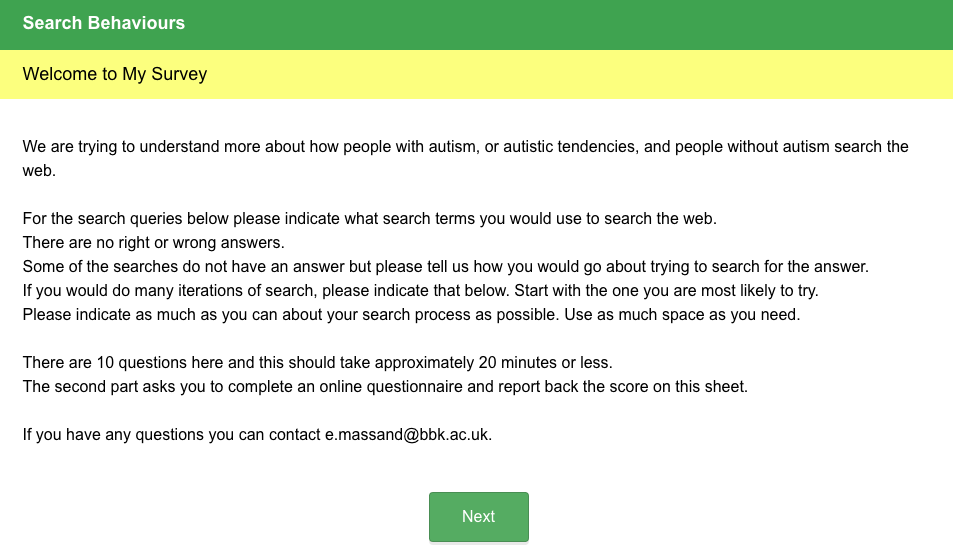
\includegraphics[scale=0.5]{survey1}\\
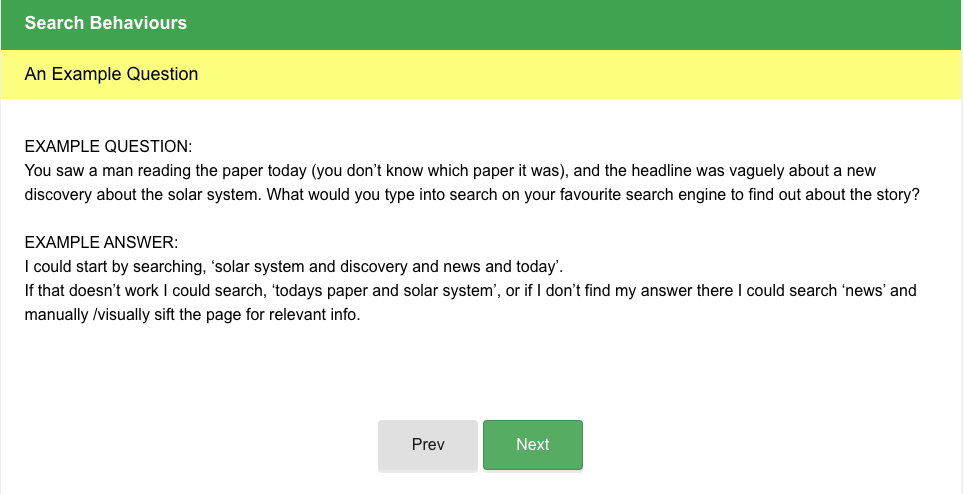
\includegraphics[scale=0.5]{survey2}\\
\end{center}
\end{figure}
\newpage
\begin{figure}[H]
\begin{center}
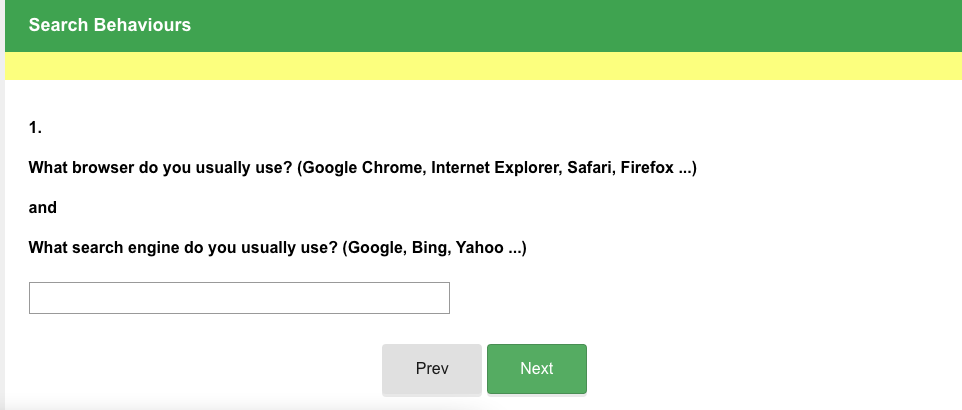
\includegraphics[scale=0.5]{survey3}\\
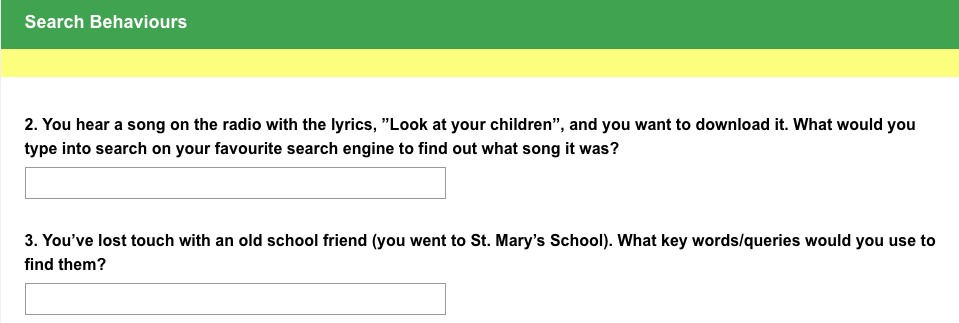
\includegraphics[scale=0.5]{survey4}\\
\end{center}
\end{figure}
\newpage
\begin{figure}[H]
\begin{center}
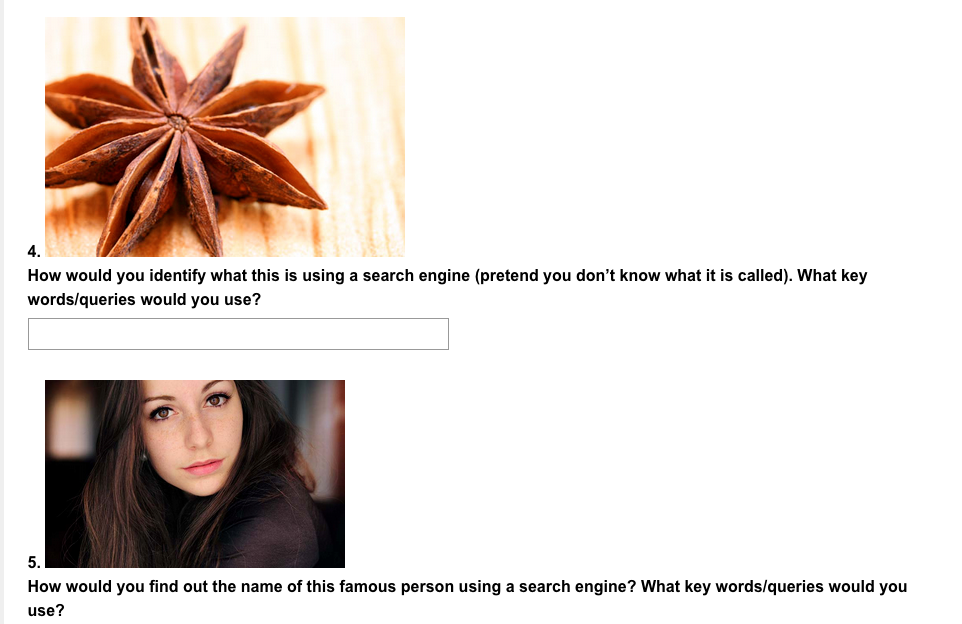
\includegraphics[scale=0.5]{survey5}\\
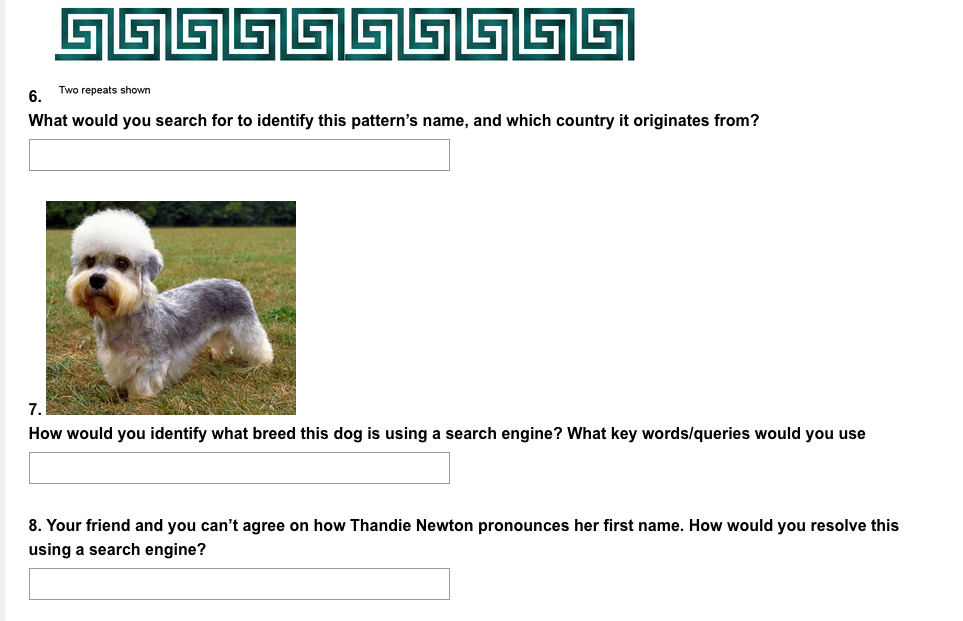
\includegraphics[scale=0.5]{survey6}\\
\end{center}
\end{figure}

\newpage
\begin{figure}[H]
\begin{center}
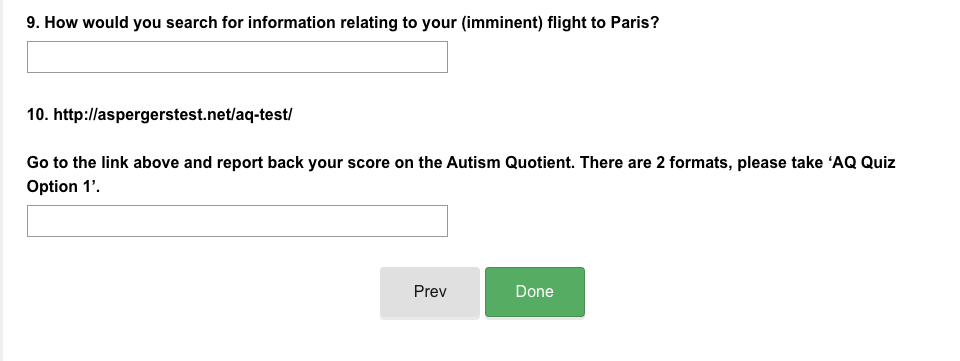
\includegraphics[scale=0.5]{survey7}\\
\caption{Search Query Survey on Surveymonkey.com \cite{surveymonkey}}
\end{center}
\end{figure}

\newpage
\subsection{Questions on the Autism Spectrum Quotient \cite{Baron Cohen et al}} \label{AQ}

Participants are asked to read each statement very carefully and rate how strongly they agree or disagree with the statement (Strongly Disagree, Slightly Disagree, Slightly Agree, or, Strongly Agree).  \\
\hspace{1cm}

I prefer to do things with others rather than on my own.\\
I prefer to do things the same way over and over again.\\
If I try to imagine something, I find it very easy to create a picture in my mind.\\
I frequently get so strongly absorbed in one thing that I lose sight of other things.\\
I often notice small sounds when others do not.\\
I usually notice car number plates or similar strings of information.\\
Other people frequently tell me that what I’ve said is impolite, even though I think it is polite.\\
When I’m reading a story, I can easily imagine what the characters might look like.\\
I am fascinated by dates.\\
In a social group, I can easily keep track of several different people’s conversations.\\
I find social situations easy.\\
I tend to notice details that others do not.\\
I would rather go to a library than a party.\\
I find making up stories easy.\\
I find myself drawn more strongly to people than to things.\\
I tend to have very strong interests which I get upset about if I can’t pursue.\\
I enjoy social chit-chat.\\
When I talk, it isn’t always easy for others to get a word in edgeways.\\
I am fascinated by numbers.\\
When I’m reading a story, I find it difficult to work out the characters’ intentions.\\
I don’t particularly enjoy reading fiction.\\
I find it hard to make new friends.\\
I notice patterns in things all the time.\\
I would rather go to the theatre than a museum.\\
It does not upset me if my daily routine is disturbed.\\
I frequently find that I don’t know how to keep a conversation going.\\
I find it easy to “read between the lines” when someone is talking to me.\\
I usually concentrate more on the whole picture, rather than the small details.\\
I am not very good at remembering phone numbers.\\
I don’t usually notice small changes in a situation, or a person’s appearance.\\
I know how to tell if someone listening to me is getting bored.\\
I find it easy to do more than one thing at once.\\
When I talk on the phone, I’m not sure when it’s my turn to speak.\\
I enjoy doing things spontaneously.\\
I am often the last to understand the point of a joke.\\
I find it easy to work out what someone is thinking or feeling just by looking at their face.\\
If there is an interruption, I can switch back to what I was doing very quickly. \\
I am good at social chit-chat.\\
People often tell me that I keep going on and on about the same thing.\\
When I was young, I used to enjoy playing games involving pretending with other children.\\
I like to collect information about categories of things (e.g. types of car, types of bird, types of train, types of plant, etc.).\\
I find it difficult to imagine what it would be like to be someone else.\\
I like to plan any activities I participate in carefully.\\
I enjoy social occasions.\\
I find it difficult to work out people’s intentions.\\
New situations make me anxious.\\
I enjoy meeting new people.\\
I am a good diplomat.\\
I am not very good at remembering people’s date of birth.\\
I find it very easy to play games with children that involve pretending.\\

\end{document}